\section{Project Planning}
		\subsection{Gantt Chart}
		\begin{center}
			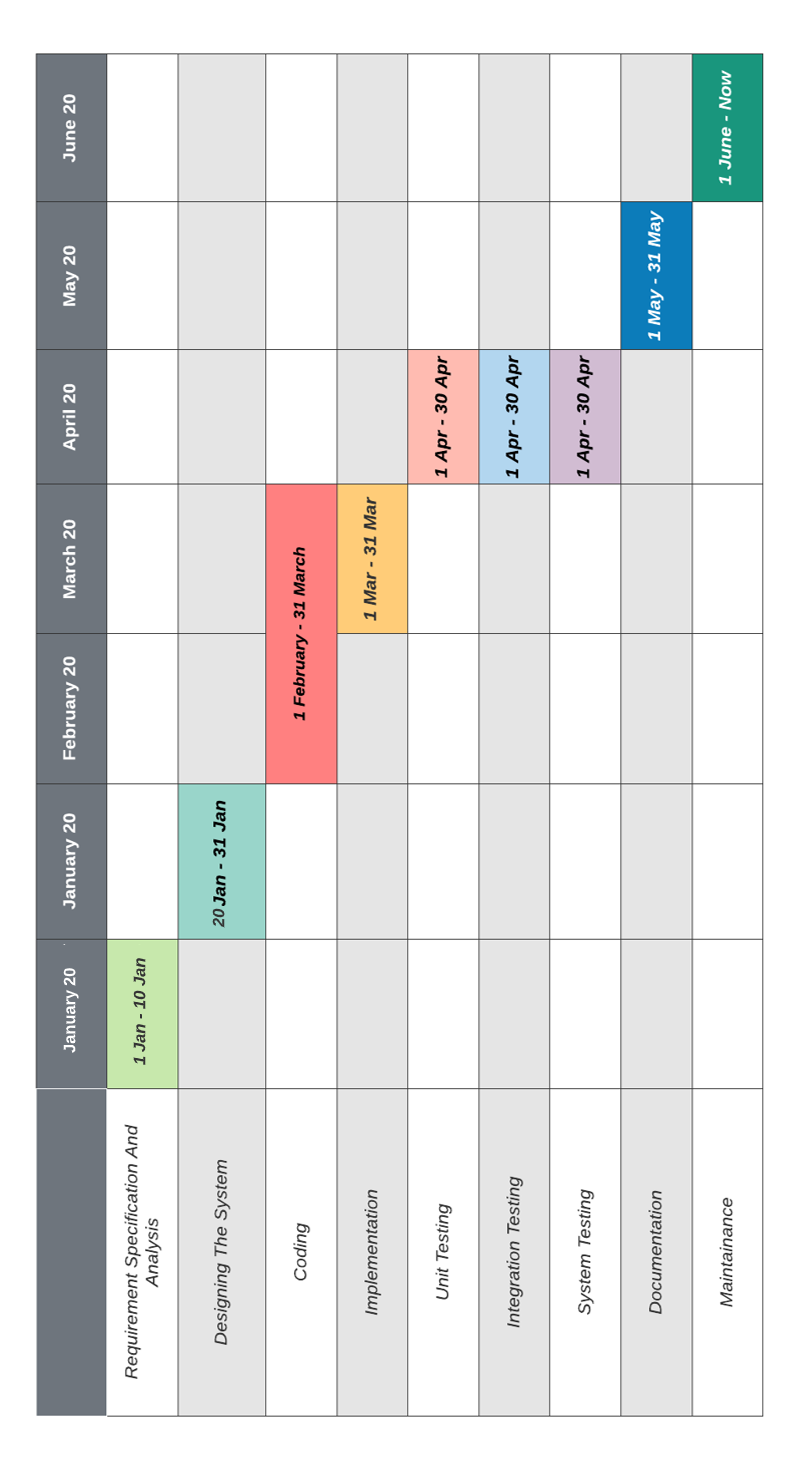
\includegraphics[width=8cm]{gc.png}
		\end{center}
		\subsection{Data Flow Diagram}
		The data Flow diagram is a graphical representation of the flow of data throughout the information system. Data flow diagrams illustrate how data is processed by a system in terms of inputs and outputs. On a DFD, data items flow from an external data source or an internal data store to an internal data store or an external data sink, via an internal process. 
		\vs
		A DFD provides no information about the timing of processes, or about whether processes will operate in sequence or parallel. It is therefore quite different from a flowchart, which shows the flow of control through an algorithm, allowing a reader to determine what operations will be performed, in what order, and under what circumstances, but not what kinds of data will be input to and output from the system, nor where the data will come from and go to, nor where the data will be stored.
		\vs
		The following notations are used to represent the operational flow in a system -
		\vs
		\bgroup
			\def\arraystretch{2}%
			\begin{center}
			\begin{tabular}{|c|m{3cm}|p{8cm}|}
				\hline
				\textbf{Name} & \textbf{Notation} & \textbf{Role} \\
				\hline
				Process & \parbox[c]{0.5cm}{
\includegraphics[width=2cm]{oval.png}} & Transforms incoming data flow to output data flow \\
				\hline
				Store & \parbox[c]{1cm}{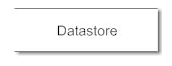
\includegraphics[width=3cm]{ds.png}} & Repositories of data in the
				system \\
				\hline
				Dataflow & \parbox[c]{1cm}{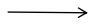
\includegraphics[width=3cm]{df.png}} & Dataflow are pipelines
				through which packets of
				information flow \\
				\hline
				External Entity & \parbox[c]{1em}{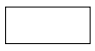
\includegraphics[width=2cm]{ee.png}} & External entities are objects
				outside the system, with which the system communicates. \\
				\hline
			\end{tabular}
			\end{center}
		\egroup
		\pagebreak
		\subsubsection{Context Level Data Flow Diagram}
		\begin{center}
			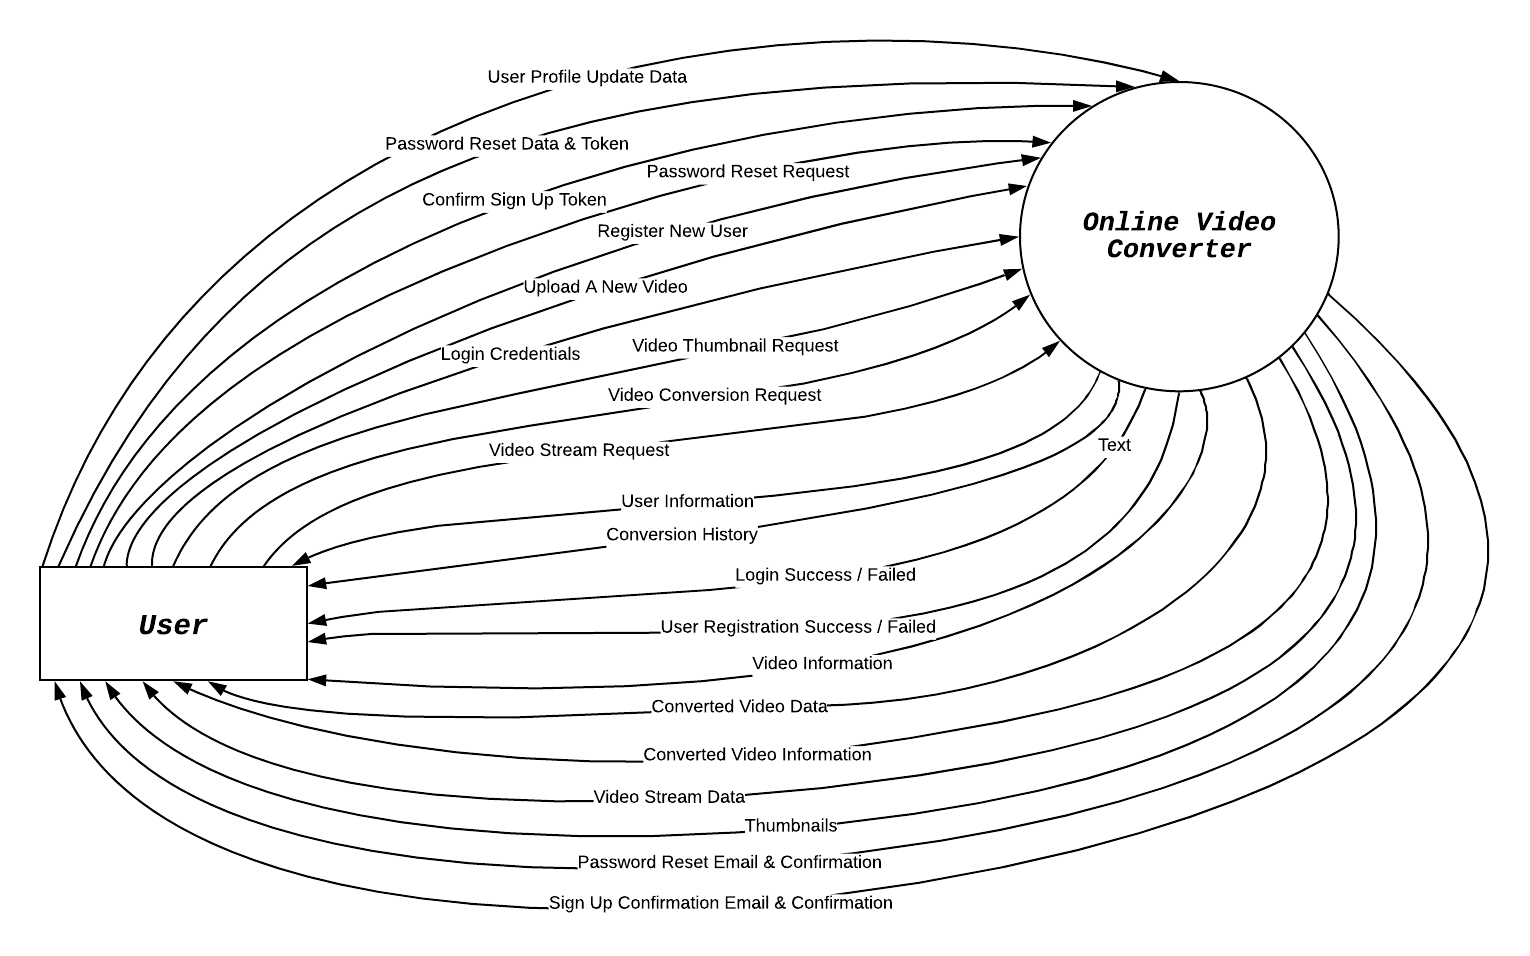
\includegraphics[width=24cm,angle=90]{ctx.png}
		\end{center}
		\pagebreak
		\subsubsection{Level-1 Data Flow Diagram}
		\begin{center}
			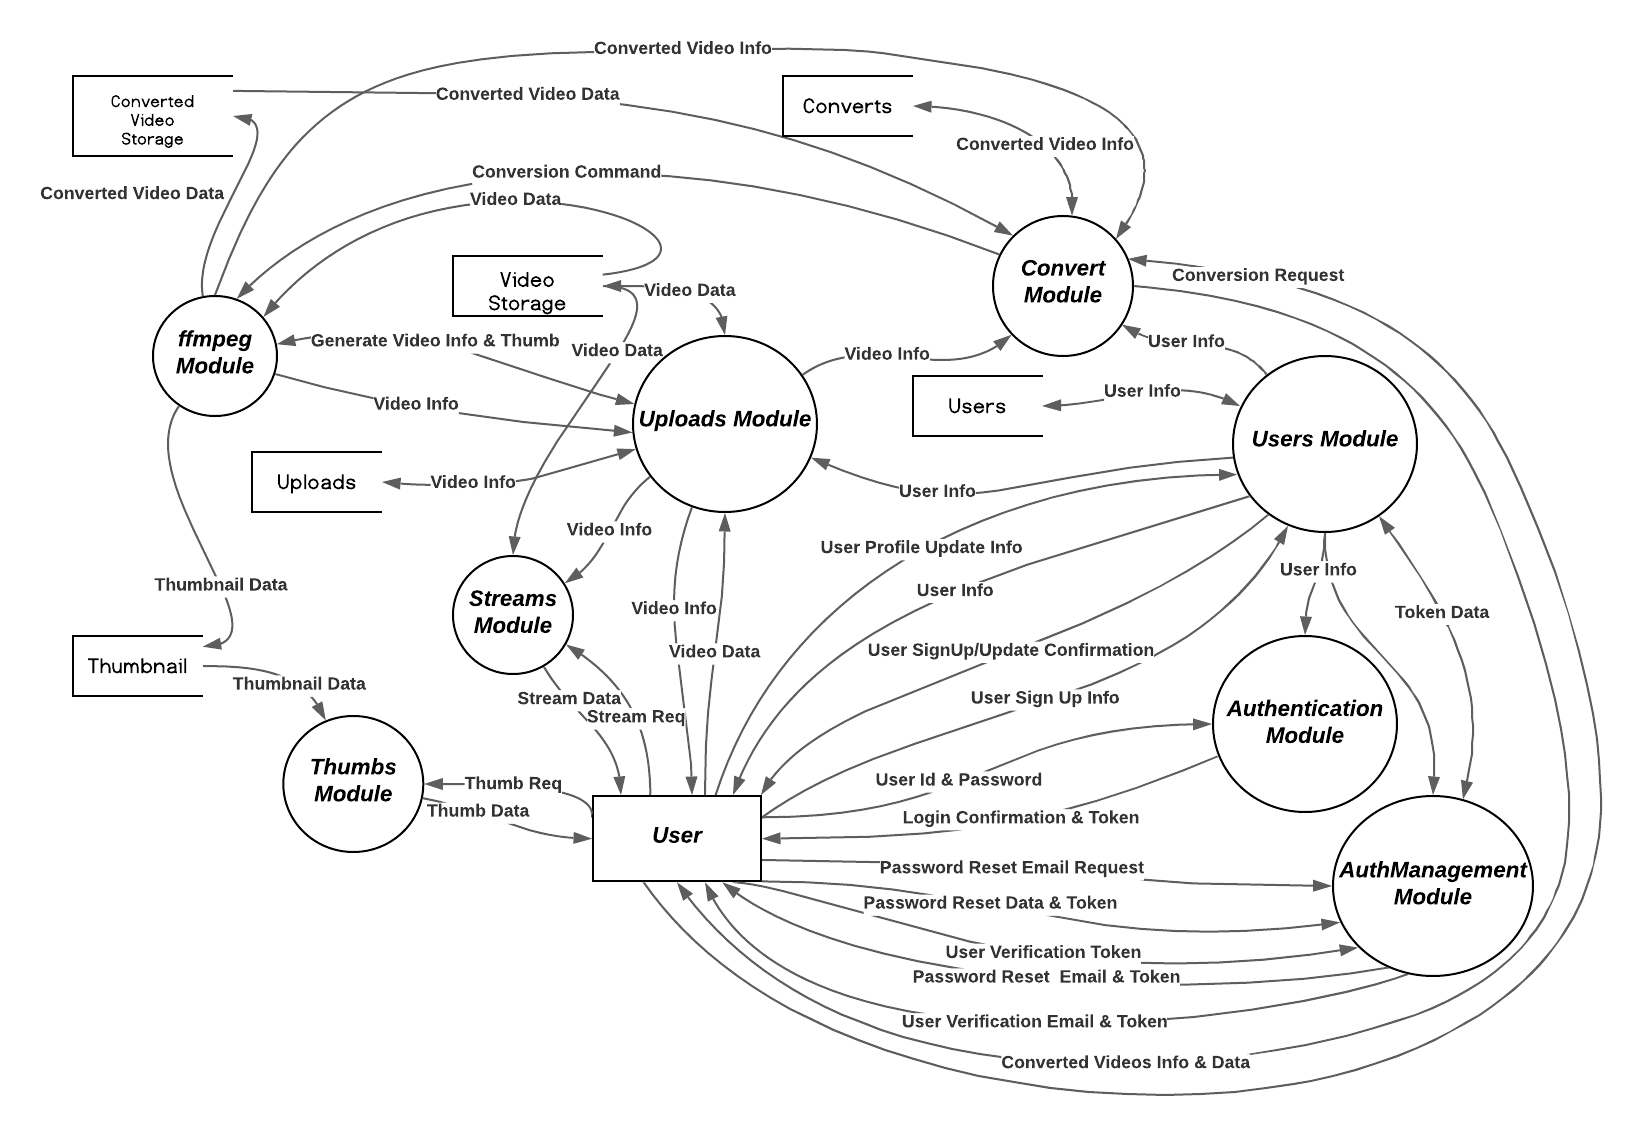
\includegraphics[width=25cm,angle=90]{dfd.png}
		\end{center}	
	\subsection{Entity-Relationship Diagram}	
	\vs
	An entity-relationship diagram describes interrelated things of interest in a specific domain of knowledge. A basic ER model consists of entity types and specifies relationships that can exist between entities.
	\vs
	An ER diagram usually consists of the following:
	\begin{itemize}
	\item 
	\textbf{\large Entity}
	
	Entities are represented through rectangles. Rectangles are named with the entity set they represent. 
	\item 
	\textbf{\large Attributes}
	
	Attributes are the properties of entities. Attributes are represented through ellipses. Every ellipse represents one attribute and is directly connected to its entity (rectangle). If the attributes are {\em composite}, they are further divided into a tree-like structure. Every node is then connected to its attribute. That is, composite attributes are represented by ellipses that are connected with an ellipse. 
	\begin{itemize}
		\item \textbf{Multivalued} attributes are depicted by double ellipses.
		\item \textbf{Derived} attributes are depicted by dashed ellipse.
	\end{itemize}
	\item 
	\textbf{\large Relationship}
	
	Relationships are represented by a diamond-shaped box. The name of the relationship is written inside the diamond-box. All the entities (rectangles) participating in a relationship, are connected to it by a line. 
	\begin{itemize}
		\item \textbf{\large Binary Relationship and Cardinality}
		
		A relationship where two entities are participating is called a binary relationship. Cardinality is the number of instances of an entity from a relation that can be associated with the relation.
		
		\begin{itemize}
			\item
			\textbf{One-To-One: }When only one instance of an entity is associated with the relationship, it is marked as '1:1'. The following image reflects that only one instance of each entity should be associated with the relationship. It depicts a one-to-one relationship.
			\vs
			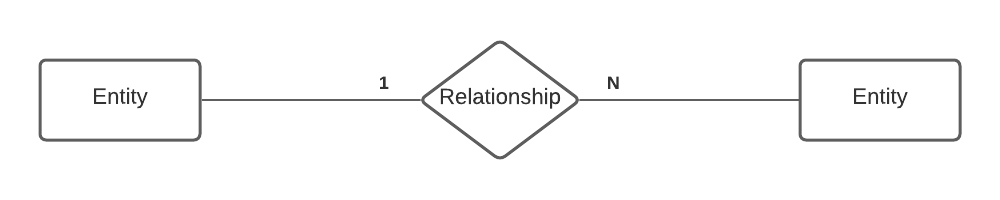
\includegraphics[width=14cm]{121.png}
			\vs
			\item
			\textbf{Many-To-One: }When more than one instance of an entity is associated with the relationship, it is marked as 'N:1'. The following image reflects that more than one instance of an entity on the left and only one instance of an entity on the right can be associated with the relationship. It depicts a many-to-one relationship.
			\vs
			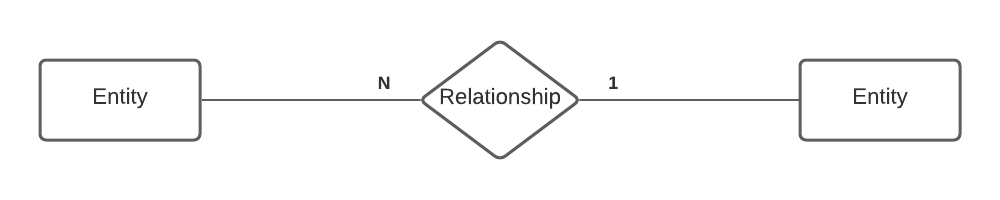
\includegraphics[width=14cm]{m21.png}
			\vs
			\item
			\textbf{Many-To-Many: }The following image reflects that more than one instance of an entity on the left and more than one instance of an entity on the right can be associated with the relationship. It depicts a many-to-many relationship.
			\vs
			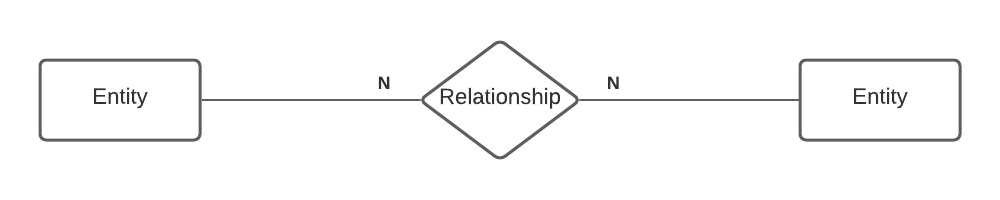
\includegraphics[width=14cm]{m2m.png}
		\end{itemize}
	\end{itemize}
	\end{itemize}
	\pagebreak
	\begin{center}
		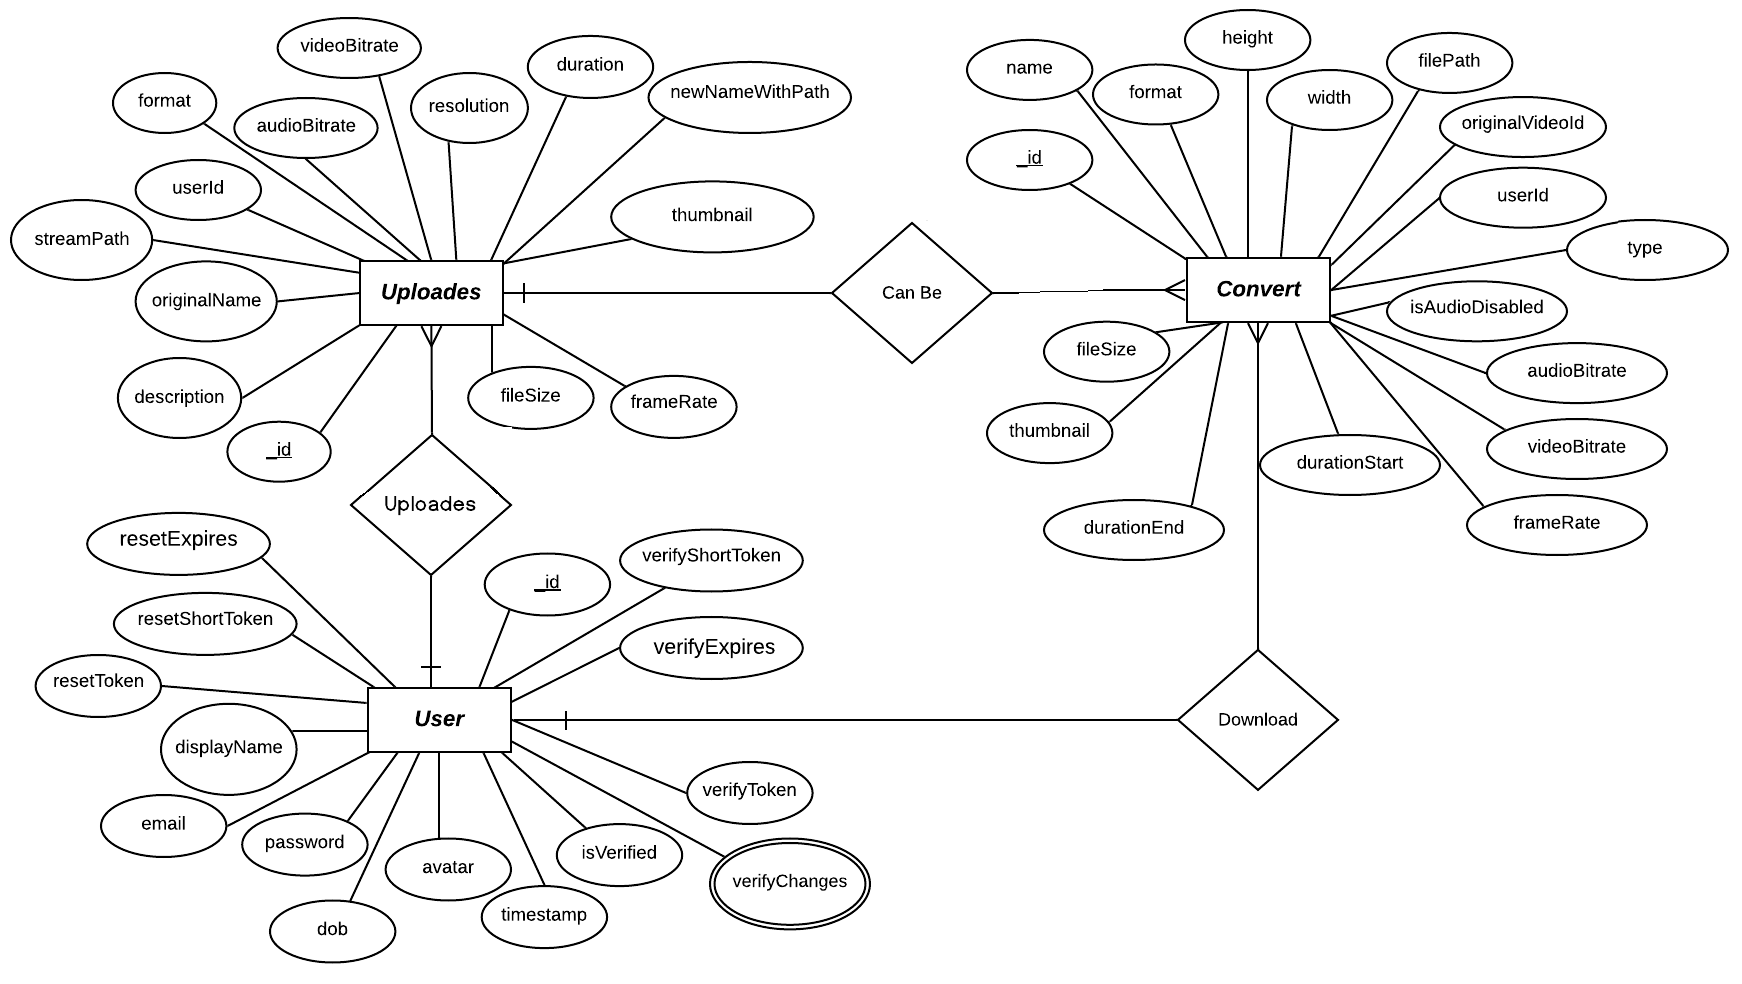
\includegraphics[width=25cm,angle=90]{er.png}
	\end{center}